\documentclass[11pt,a4paper]{scrartcl}
\typearea{12}
\usepackage{graphicx}
\usepackage{pstricks}
\usepackage{listings}
\lstset{language=python}
\pagestyle{headings}
\markright{Computation Neuroscience - 7 vision}

\usepackage{tikz}
%\usepackage{tikzscale}
\usepackage{pgfplots}
\usepackage{color}
\usepackage{pgf}
\usepackage[utf8]{inputenc}
\usetikzlibrary{arrows,automata}
\usetikzlibrary{positioning}


\begin{document}

\section*{Vision - removed material}
This is an earlier, longer, but no less confusing version of the confusing aside.

\subsubsection*{Confusing aside - rate versus reconstruction}
The slightly confusing thing here is that we are moving between the linear model and the reconstruction. We do this all the time with vectors:
\begin{equation}
\textbf{v}=v_1\textbf{i}+v_2\textbf{j}+v_3\textbf{k}
\end{equation}
is the reconstruction where the corresponding project, for example
\begin{equation}
v_1=\textbf{v}\cdot\textbf{i}
\end{equation}
is like the linear model. In other words, in the construction we make
the vector out of the components and the basis vectors, in the
projection we work out the components using the basis vectors. The
situation in this case is pretty striaght-forward, because the basis
vectors are orthonormal
\begin{equation}
\textbf{i}\cdot\textbf{j}=\textbf{j}\cdot\textbf{k}=\textbf{k}\cdot\textbf{i}=0
\end{equation}
and
\begin{equation}
\textbf{i}\cdot\textbf{i}=\textbf{j}\cdot\textbf{j}=\textbf{k}\cdot\textbf{k}=1
\end{equation}
the same basis vector appears in the reconstruction and the
projection: the coeffient $v_1$ of $\textbf{i}$ in the reconstruction
is the projection of $\textbf{v}$ onto $\textbf{i}$. However, in the
case of vision the basis elements, the $W^s_{ij}$ and $w^s_{ij}$ are
not orthonormal and therefore are not the same, working out the
relationship between involves vectorizing the matrix indices $i$ and
$j$, so we won't go into it here, morally one is the inverse transpose
of the other. In fact, here we will consider an example where the
dimensions are different, where the image patches are $3\times 3$ but
there are only six features, so $s=1\ldots 6$. This means that the
reconstructed image may not be equal the original image and will just
be an approximation to it.

As an example, lets have
\begin{center}
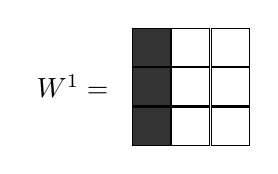
\begin{tikzpicture}
\node at (-1,0.5){$W^1=$};
\node at (0,0)[rectangle,text width=0.25cm,text height=0.25cm,draw=black,fill=black!80,align=center](00){};
\node at (0,0.5)[rectangle,text width=0.25cm,text height=0.25cm,draw=black,fill=black!80,align=center](01){};
\node at (0,1)[rectangle,text width=0.25cm,text height=0.25cm,draw=black,fill=black!80,align=center](02){};
\node at (0.5,0)[rectangle,text width=0.25cm,text height=0.25cm,draw=black,fill=black!0,align=center](10){};
\node at (0.5,0.5)[rectangle,text width=0.25cm,text height=0.25cm,draw=black,fill=black!0,align=center](11){};
\node at (0.5,1)[rectangle,text width=0.25cm,text height=0.25cm,draw=black,fill=black!0,align=center](12){};
\node at (1,0)[rectangle,text width=0.25cm,text height=0.25cm,draw=black,fill=black!0,align=center](20){};
\node at (1,0.5)[rectangle,text width=0.25cm,text height=0.25cm,draw=black,fill=black!0,align=center](21){};
\node at (1,1)[rectangle,text width=0.25cm,text height=0.25cm,draw=black,fill=black!0,align=center](22){};
\end{tikzpicture}
\quad
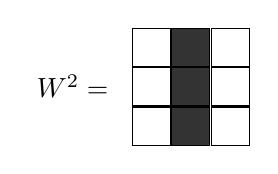
\begin{tikzpicture}
\node at (-1,0.5){$W^2=$};
\node at (0,0)[rectangle,text width=0.25cm,text height=0.25cm,draw=black,fill=black!0,align=center](00){};
\node at (0,0.5)[rectangle,text width=0.25cm,text height=0.25cm,draw=black,fill=black!0,align=center](01){};
\node at (0,1)[rectangle,text width=0.25cm,text height=0.25cm,draw=black,fill=black!0,align=center](02){};
\node at (0.5,0)[rectangle,text width=0.25cm,text height=0.25cm,draw=black,fill=black!80,align=center](10){};
\node at (0.5,0.5)[rectangle,text width=0.25cm,text height=0.25cm,draw=black,fill=black!80,align=center](11){};
\node at (0.5,1)[rectangle,text width=0.25cm,text height=0.25cm,draw=black,fill=black!80,align=center](12){};
\node at (1,0)[rectangle,text width=0.25cm,text height=0.25cm,draw=black,fill=black!0,align=center](20){};
\node at (1,0.5)[rectangle,text width=0.25cm,text height=0.25cm,draw=black,fill=black!0,align=center](21){};
\node at (1,1)[rectangle,text width=0.25cm,text height=0.25cm,draw=black,fill=black!0,align=center](22){};
\end{tikzpicture}
\quad
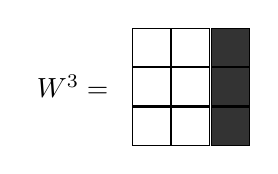
\begin{tikzpicture}
\node at (-1,0.5){$W^3=$};
\node at (0,0)[rectangle,text width=0.25cm,text height=0.25cm,draw=black,fill=black!0,align=center](00){};
\node at (0,0.5)[rectangle,text width=0.25cm,text height=0.25cm,draw=black,fill=black!0,align=center](01){};
\node at (0,1)[rectangle,text width=0.25cm,text height=0.25cm,draw=black,fill=black!0,align=center](02){};
\node at (0.5,0)[rectangle,text width=0.25cm,text height=0.25cm,draw=black,fill=black!0,align=center](10){};
\node at (0.5,0.5)[rectangle,text width=0.25cm,text height=0.25cm,draw=black,fill=black!0,align=center](11){};
\node at (0.5,1)[rectangle,text width=0.25cm,text height=0.25cm,draw=black,fill=black!0,align=center](12){};
\node at (1,0)[rectangle,text width=0.25cm,text height=0.25cm,draw=black,fill=black!80,align=center](20){};
\node at (1,0.5)[rectangle,text width=0.25cm,text height=0.25cm,draw=black,fill=black!80,align=center](21){};
\node at (1,1)[rectangle,text width=0.25cm,text height=0.25cm,draw=black,fill=black!80,align=center](22){};
\end{tikzpicture}
\end{center}
\begin{center}
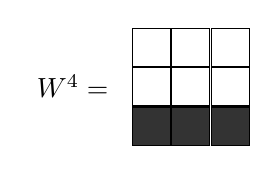
\begin{tikzpicture}
\node at (-1,0.5){$W^4=$};
\node at (0,0)[rectangle,text width=0.25cm,text height=0.25cm,draw=black,fill=black!80,align=center](00){};
\node at (0,0.5)[rectangle,text width=0.25cm,text height=0.25cm,draw=black,fill=black!0,align=center](01){};
\node at (0,1)[rectangle,text width=0.25cm,text height=0.25cm,draw=black,fill=black!0,align=center](02){};
\node at (0.5,0)[rectangle,text width=0.25cm,text height=0.25cm,draw=black,fill=black!80,align=center](10){};
\node at (0.5,0.5)[rectangle,text width=0.25cm,text height=0.25cm,draw=black,fill=black!0,align=center](11){};
\node at (0.5,1)[rectangle,text width=0.25cm,text height=0.25cm,draw=black,fill=black!0,align=center](12){};
\node at (1,0)[rectangle,text width=0.25cm,text height=0.25cm,draw=black,fill=black!80,align=center](20){};
\node at (1,0.5)[rectangle,text width=0.25cm,text height=0.25cm,draw=black,fill=black!0,align=center](21){};
\node at (1,1)[rectangle,text width=0.25cm,text height=0.25cm,draw=black,fill=black!0,align=center](22){};
\end{tikzpicture}
\quad
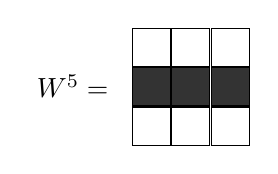
\begin{tikzpicture}
\node at (-1,0.5){$W^5=$};
\node at (0,0)[rectangle,text width=0.25cm,text height=0.25cm,draw=black,fill=black!0,align=center](00){};
\node at (0,0.5)[rectangle,text width=0.25cm,text height=0.25cm,draw=black,fill=black!80,align=center](01){};
\node at (0,1)[rectangle,text width=0.25cm,text height=0.25cm,draw=black,fill=black!0,align=center](02){};
\node at (0.5,0)[rectangle,text width=0.25cm,text height=0.25cm,draw=black,fill=black!0,align=center](10){};
\node at (0.5,0.5)[rectangle,text width=0.25cm,text height=0.25cm,draw=black,fill=black!80,align=center](11){};
\node at (0.5,1)[rectangle,text width=0.25cm,text height=0.25cm,draw=black,fill=black!0,align=center](12){};
\node at (1,0)[rectangle,text width=0.25cm,text height=0.25cm,draw=black,fill=black!0,align=center](20){};
\node at (1,0.5)[rectangle,text width=0.25cm,text height=0.25cm,draw=black,fill=black!80,align=center](21){};
\node at (1,1)[rectangle,text width=0.25cm,text height=0.25cm,draw=black,fill=black!0,align=center](22){};
\end{tikzpicture}
\quad
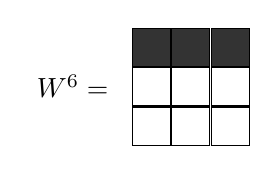
\begin{tikzpicture}
\node at (-1,0.5){$W^6=$};
\node at (0,0)[rectangle,text width=0.25cm,text height=0.25cm,draw=black,fill=black!0,align=center](00){};
\node at (0,0.5)[rectangle,text width=0.25cm,text height=0.25cm,draw=black,fill=black!0,align=center](01){};
\node at (0,1)[rectangle,text width=0.25cm,text height=0.25cm,draw=black,fill=black!80,align=center](02){};
\node at (0.5,0)[rectangle,text width=0.25cm,text height=0.25cm,draw=black,fill=black!0,align=center](10){};
\node at (0.5,0.5)[rectangle,text width=0.25cm,text height=0.25cm,draw=black,fill=black!0,align=center](11){};
\node at (0.5,1)[rectangle,text width=0.25cm,text height=0.25cm,draw=black,fill=black!80,align=center](12){};
\node at (1,0)[rectangle,text width=0.25cm,text height=0.25cm,draw=black,fill=black!0,align=center](20){};
\node at (1,0.5)[rectangle,text width=0.25cm,text height=0.25cm,draw=black,fill=black!0,align=center](21){};
\node at (1,1)[rectangle,text width=0.25cm,text height=0.25cm,draw=black,fill=black!80,align=center](22){};
\end{tikzpicture}
\end{center}
where the almost-black corresponds to one and white to zero, so put another way
\begin{equation}
[W^1_{ij}]=\left(\begin{array}{lll}1&0&0\\1&0&0\\1&0&0\end{array}\right)
\end{equation}
Now consider the example visual input
\begin{center}
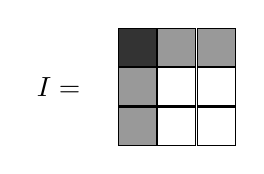
\begin{tikzpicture}
\node at (-1,0.5){$I=$};
\node at (0,0)[rectangle,text width=0.25cm,text height=0.25cm,draw=black,fill=black!40,align=center](00){};
\node at (0,0.5)[rectangle,text width=0.25cm,text height=0.25cm,draw=black,fill=black!40,align=center](01){};
\node at (0,1)[rectangle,text width=0.25cm,text height=0.25cm,draw=black,fill=black!80,align=center](02){};
\node at (0.5,0)[rectangle,text width=0.25cm,text height=0.25cm,draw=black,fill=black!0,align=center](10){};
\node at (0.5,0.5)[rectangle,text width=0.25cm,text height=0.25cm,draw=black,fill=black!0,align=center](11){};
\node at (0.5,1)[rectangle,text width=0.25cm,text height=0.25cm,draw=black,fill=black!40,align=center](12){};
\node at (1,0)[rectangle,text width=0.25cm,text height=0.25cm,draw=black,fill=black!0,align=center](20){};
\node at (1,0.5)[rectangle,text width=0.25cm,text height=0.25cm,draw=black,fill=black!0,align=center](21){};
\node at (1,1)[rectangle,text width=0.25cm,text height=0.25cm,draw=black,fill=black!40,align=center](22){};
\end{tikzpicture}
\end{center}
This would correspond to $a=(0.5,0,0,0,0,0.5)$ or
\begin{center}
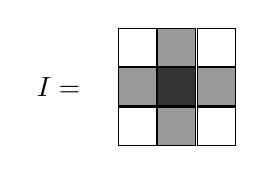
\begin{tikzpicture}
\node at (-1,0.5){$I=$};
\node at (0,0)[rectangle,text width=0.25cm,text height=0.25cm,draw=black,fill=black!0,align=center](00){};
\node at (0,0.5)[rectangle,text width=0.25cm,text height=0.25cm,draw=black,fill=black!40,align=center](01){};
\node at (0,1)[rectangle,text width=0.25cm,text height=0.25cm,draw=black,fill=black!0,align=center](02){};
\node at (0.5,0)[rectangle,text width=0.25cm,text height=0.25cm,draw=black,fill=black!40,align=center](10){};
\node at (0.5,0.5)[rectangle,text width=0.25cm,text height=0.25cm,draw=black,fill=black!80,align=center](11){};
\node at (0.5,1)[rectangle,text width=0.25cm,text height=0.25cm,draw=black,fill=black!40,align=center](12){};
\node at (1,0)[rectangle,text width=0.25cm,text height=0.25cm,draw=black,fill=black!0,align=center](20){};
\node at (1,0.5)[rectangle,text width=0.25cm,text height=0.25cm,draw=black,fill=black!40,align=center](21){};
\node at (1,1)[rectangle,text width=0.25cm,text height=0.25cm,draw=black,fill=black!0,align=center](22){};
\end{tikzpicture}
\end{center}
corresponds to $a=(0,0.5,0,0,0.5,0)$ whereas
\begin{center}
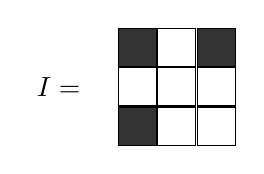
\begin{tikzpicture}
\node at (-1,0.5){$I=$};
\node at (0,0)[rectangle,text width=0.25cm,text height=0.25cm,draw=black,fill=black!80,align=center](00){};
\node at (0,0.5)[rectangle,text width=0.25cm,text height=0.25cm,draw=black,fill=black!0,align=center](01){};
\node at (0,1)[rectangle,text width=0.25cm,text height=0.25cm,draw=black,fill=black!80,align=center](02){};
\node at (0.5,0)[rectangle,text width=0.25cm,text height=0.25cm,draw=black,fill=black!0,align=center](10){};
\node at (0.5,0.5)[rectangle,text width=0.25cm,text height=0.25cm,draw=black,fill=black!0,align=center](11){};
\node at (0.5,1)[rectangle,text width=0.25cm,text height=0.25cm,draw=black,fill=black!0,align=center](12){};
\node at (1,0)[rectangle,text width=0.25cm,text height=0.25cm,draw=black,fill=black!0,align=center](20){};
\node at (1,0.5)[rectangle,text width=0.25cm,text height=0.25cm,draw=black,fill=black!0,align=center](21){};
\node at (1,1)[rectangle,text width=0.25cm,text height=0.25cm,draw=black,fill=black!80,align=center](22){};
\end{tikzpicture}
\end{center}
lies outside the six-dimensional subspace spanned by the features.


\end{document}

